\chapter{The DORIS System}
\label{ch:doris-system}

\section{DORIS Observation Equation}
\label{sec:doppler-effect}

In the following, we will use the notation:
\begin{description}
  \item[$\tau$] proper time, e.g. a time tag in the time-scale of the receiver
  \item[$t$] coordinate time, e.g. a time tag in TAI
\end{description}

$N_{DOP}$, aka the \emph{Doppler measurement} is the count, by the receiver 
electronics, of the number of cycles of the difference $N_e$ (cycles sent by the 
emitter, $N_e=f_e \Delta \tau_e$) and $N_r$ (cycles generated by the receiver, 
$N_r=f_r \Delta \tau_r$). In practice, this is computed by the difference of two, 
consecutive \texttt{L2GHz} observation values (for the same beacon) in the RINEX file.
This difference is given in the proper time-scale of the receiver.

Note that:
\begin{equation}
  \begin{split}
    N_{DOP} & = N_e - N_r\\
            & = f_e \Delta\tau_e - f_r \Delta\tau_r
  \end{split}
\end{equation}

In an ``ideal world'' (that is ignoring time-scales, relativity, atmospheric 
refraction, etc), this measurement differentiated by the time interval between the 
two measurements, would give the \emph{range-rate}, i.e. the relative becon-to-satellite 
velocity.

\textbf{Range Rate}\\
\label{range-rate}
Suppose that the two consecutive measurements are performed at $\tau_{r_1}$ 
and $\tau_{r_2}$ respectively, at the receiver proper time. We must compute the 
``\emph{theoretical}'' range-rate value (to compare it with the value observed).
According to \cite{Montenbruck2000}, the formula for computing range-rate is:
\begin{equation}
  \dot{\rho} = \frac{\rho_{\tau_{r_2}} - \rho_{\tau_{r_1}}}{\tau_{r_2} - \tau_{r_1}}
\end{equation}
In the implementation, the formula is computed using \emph{topocentric} vectors 
(with origin at the beacon). Hence $\rho_{\tau_{r_1}}$ and $\rho_{\tau_{r_2}}$ are 
actualy $\rho_{\tau_{r_1}}^{enu}$ and $\rho_{\tau_{r_2}}^{enu}$.

Note, that the above is different from the \emph{instataneous} range rate, 
which is computed via (\cite{Montenbruck2000})
\begin{equation}
  \dot{\rho} = \dot{s} = \frac{\bm{s} \bm{\dot{s}}}{s}
\end{equation}

\textbf{Beacon Nominal Frequencies}\\
\label{beacon-nominal-frequencies}
The RINEX file contains a \emph{station frequency shift factor} for each of the 
beacons included. This is used to compute the ``nominal'' frequencies of the 
beacon/emitter. Usually, this shift factor is just $0$, but it can be an integer 
$k \neq 0$. The frequencies are computed as:
\begin{equation}
  \begin{align}
    L_{2GHz}   &= 543 \cdot F_0 \left( \frac{3}{4} + \frac{87\cdot k}{5 \cdot 2^{26}} \right) \\
    L_{400MHz} &= 107 \cdot F_0 \left( \frac{3}{4} + \frac{87\cdot k}{5 \cdot 2^{26}} \right) 
  \end{align}
\end{equation}
where $F_0 = 5e6 \text{ Hz}$ the USO frequency.

\textbf{Measurement Flags}\\
\label{measurement-flags}
Each observation (on each frequency) in the RINEX file is marked with two ``flags'', 
aka two distinct characters that follow the observation value and flag important 
events if any. Here, we will exclude observations if the following conditions are true:
\begin{description}
  \item[\texttt{L2GHz} or \texttt{L400MHz}] measurement is a ``central frequency'' 
  measurement (that is the first flag is an \texttt{1})
  \item[\texttt{L2GHz} or \texttt{L400MHz}] measurement is marked as discontinuity, 
  i.e. Loss-of-Lock has occured (that is the seconds flag is an \texttt{1})
  \item[power-level \texttt{W}] measurement (on either of the frequencies) flags 
  a beacon on restart mode (first flag is an \texttt{1})
\end{description}

\textbf{Ionospheric Refraction}
\label{ionospheric-refraction}
For each observation, the ionosphere-induced delay is computed using both 
(carrier) phase measurements. The correction, for each observation, is: 
(\cite{lemoine-2016}):
\begin{equation}
  L_{iono-free-2GHz} = L_{2GHz} 
    + \frac{L_{2GHz} - \sqrt \gamma L_{400MHz}}{\gamma - 1} 
    \text{ in [cycles]}
\end{equation}
For the observation equation, we should differentiate the ionospheric delays on 
(the) two consecutive observations, to compute $\Delta u_{ION}$. Thus,
\begin{equation}
  \Delta u_{ION} = \frac{c}{f_{rN}} \left( L_{iono-free-2GHz}^{\tau_{r_2}} 
    - L_{iono-free-2GHz}^{\tau_{r_1}} \right) / (\tau_{r_2} - \tau_{r_1})
    \text{ in [m/sec]}
\end{equation}
Note that the above meas that we are now referencing a ``iono-free'' phase center, 
different than the L2GHz phase center.

\textbf{Tropospheric Refraction}
\label{tropospheric-refraction}
For each observation we have to compute the tropospheric delay. This is done using 
the GPT3/VMF3 model. GPT3 uses a grid to compute values for various atmospheric 
parameters (e.g. pressure, temperature, etc). VMF3 computes mapping functions values 
$mf_{el}^{wet}$ and $mf_{el}^{hydrostatic}$ for given elevation/zenith angles.
For the hydrostatic zenith path delay $L_{z}^{hydrostatic}$, we use the 
``refined'' Saastamoinen formula. An approximate, a-priori value for the 
respective wet delay $L_{z}^{wet}$ can be computed using the Aske \& Nordius 
formula. Finaly:
\begin{equation}
  \Delta _{trop} = L_{z}^{hyd} \cdot mf_{el}^{hyd} 
                 + L_{z}^{wet} \cdot mf_{el}^{wet} \text{ in [m]}
\end{equation}
As with the ionosphere, when considering the Doppler observation equation, we should 
get the differential correction betwee two consecutive observations,
\begin{equation}
  \begin{split}
  \label{eq:dutropo}
  \Delta u_{TRO} & = \left( \Delta _{trop}^{\tau_{r_2}} 
                  - \Delta _{trop}^{\tau_{r_1}} \right)
                    / (\tau_{r_2} - \tau_{r_1}) \\
                 & = \frac{L_{z,\tau_{r_2}}^{hyd} \cdot mf_{el,\tau_{r_2}}^{hyd} 
                   - L_{z,\tau_{r_1}}^{hyd} \cdot mf_{el,\tau_{r_1}}^{hyd} 
                   + L_{z}^{wet} \left( mf_{el,\tau_{r_2}}^{wet} - mf_{el,\tau_{r_1}}^{wet} \right)}
                   {\tau_{r_2} - \tau_{r_1}} \\
                 & \text{ in [m/sec]}
  \end{split}
\end{equation}
For every observation, a call to GPT3 is made to compute various quantities, 
that depend both on time and (beacon) coordinates. A call to VMF3 is performed 
to compute the mapping functions $mf_{el,\tau_i}^{wet}$ and $mf_{el,\tau_i}^{hyd}$.
Again, for every observation/beacon we compute the zenith hydrostatic delay 
$L_{z,\tau_i}^{hyd}$. The zenith wet delay $L_{z}^{wet}$ is considered a constant 
for one satellite pass. An a-priori value is computed using the Aske \& Nordius formula 
and the value is estimated as a (filter) parameter.

Considering \ref{eq:dutropo}, the following {\color{lime} simplified} partial 
derivatives are derived:
\begin{align}
  \frac{\partial \Delta u_{TRO}}{\partial \bm{r}_{beacon}}    
    &= \frac{\partial \Delta u_{TRO}}{\partial \bm{v}_{beacon}} = \bm{0} \\
  \frac{\partial \Delta u_{TRO}}{\partial \bm{r}_{satellite}} 
    &= \frac{\partial \Delta u_{TRO}}{\partial \bm{v}_{satellite}} = \bm{0} \\
  \frac{\partial \Delta u_{TRO}}{\partial L_{z}^{wet}} 
    &= \frac{mf_{el,\tau_{r_2}}^{wet} - mf_{el,\tau_{r_1}}^{wet}}{\tau_{r_2} - \tau_{r_1}}
\end{align}

\textbf{Relativistic Corrections}
According to \cite{lemoine-2016}, relativistic correction can be split into two 
parts, $\Delta_{rel_C}$, which is the clock correction, and $\Delta_{rel_r}$ 
which is the travel-time correction. They are given respectively by:
\begin{equation}
  \label{eq:relativistic-clock-correction}
  \Delta_{rel_C} = \frac{1}{c} \left( U_r - U_e + \frac{V_r^2 -V_e^2}{2} \right)
\end{equation}
\begin{equation}
  \Delta_{rel_r} = \frac{2\mu}{\Delta \tau _r c^2} 
    \left( \ln{\frac{R_1+R_{1'}+\rho_1}{R_1+R_{1'}-\rho_1}} 
      - \ln{\frac{R_2+R_{2'}+\rho_2}{R_2+R_{2'}-\rho_2}} \right)
\end{equation}
{\color{brown}At this point, we are only considering the relativistic clock correction!}.
In \ref{eq:relativistic-clock-correction}, the subscript \texttt{e} denotes the 
emitter which in DORIS is the beacon, which is located on the surface of the 
Earth, close to the geoid. Hence, we can use the approximation:
\begin{equation}
  U_e + V_e^2 / 2 = \mu / r_{beacon}^{ecef}
\end{equation}

On the other hand, the gravitational potential for a LEO satellite cannot be 
approximated adequately using only the fist term. Hence, we will include the 
$J_2$ term so that:
\begin{equation}
  U_r = \frac{\mu}{r_{satellite}^{ecef}} - 
    \left( 1 - \left( \frac{\alpha _e}{r_{satellite}^{ecef}} \right) ^2 
      \cdot J_2 \cdot \frac{3 \sin^{2}{\phi} -1}{2} \right)
\end{equation}
where $\alpha _e$ is the equatorial radius of the earth. The term $V_r$ is 
simply the norm of the satellite's {\color{brown}velocity vector in ECEF}.
Is this last sentence correct?

\textbf{Beacon Coordinates and Reference Points}
\label{beacon-coordiates-and-reference-points}
Beacon coordinates are extracted from the \texttt{dpod2014\_053.snx} file, and 
extrapolated to first epoch of the RINEX file. {\color{brown} Loading/Tidal site 
displacements are ot yet considered}, hence the beacon position is considered 
stable for all measurements in the RINEX file.

Because we are using iono-free 2GHz measuremets, we must ``reduce'' the beacon 
coordinates to reference the iono-free phase center. For this, we procced as 
\cite{lemoine-2016}, aka the vector from the beacon Reference Point to the
2GHz-iono-free phase center is:
\begin{equation}
  \bm{r}'_{iono-free-2GHz} = \bm{r}_{2GHz} + 
    \frac{\bm{r}_{2GHz} - \bm{r}_{400MHz}}{\gamma - 1}
\end{equation}
Note that this equation is w.r.t a topocentric reference frame.

The actual computation for this reduction is:
\begin{enumerate}
  \item transform the beacon coordinates from Cartesian ECEF to ellipsoidal ECEF
  \item compute the ECEF-to-topocentric rotation matrix $R$ (that is 
    $\bm{x}_{enu} = R \cdot \delta \bm{x}_{xyz}$)
  \item compute the iono-free-2GHz reference position as:
  \begin{equation}
    \bm{r}_{iono-free-2GHz}^{xyz} = \bm{r}_{dpod} + R^T \cdot \bm{r}'_{iono-free-2GHz}
  \end{equation}
\end{enumerate}

{\color{brown}Here we are assuming that the beacon coordinates in the SINEX 
file correspond to the antenna RP. Is that true? If DORIS is like GNSS, it 
could be that the log files contain eccentricities. Make a Python script to 
parse DORIS log files and spit beacon eccentricities.}


\textbf{Pseudocode}
\begin{enumerate}
  
  \item Extract/extrapolate all beacon coordinates from \texttt{dpod2014\_053.snx}, 
    contained in the RINEX file. These will be the reference coordinates. 
    Extrapolation is performed to the first epoch contained in the RINEX file to 
    get $\bm{r}_{e,dpod}^{ecef}$ for each beacon.

  \item For every new epoch/data-block contained in the RINEX file and taged as $t_i$ in \texttt{TAI}.
  \begin{enumerate}
    \item compute receiver/satellite ``proper'' time using the 
    \emph{receiver clock offset} correction in the block header; this will 
     be $\tau_{i}$ (note that this correction can be quite large and up to 
     1 minute!).

    \item integrate satellite orbit to get state at {\color{red} $\tau_{i}$}. 
    Transform state to ECEF, $\bm{r}_{r}^{ecef}$.

    \item for each beacon (observation set) in this, current block:
    \begin{enumerate}
      \item check observation flags (\ref{measurement-flags}). If flags are ok 
      procced, else mark as discontinuous and skip observation for this beacon.

      \item compute iono-free-2GHz reference point of the beacon 
      (\ref{beacon-coordiates-and-reference-points}), henceforth, we are going 
      to use these coordinates for the beacon: 
      $\bm{r}_{e}^{ecef} \equiv \bm{r}_{iono-free-2GHz}^{ECEF}$

      \item compute azimouth $Az$, elevation $el$ and range $\rho$, of the 
      beacon-satellite vector (performed in topocentric RF). If the elevation 
      is above some fixed value (e.g. 7 degrees) procced.

      \item compute ``nominal'' values for the beacon frequencies 
      (\ref{beacon-nominal-frequencies}) $f_{eN}$ (for 2GHz and 400MHz).

      \item compute ionospheric correction for this observation 
      (\ref{ionospheric-refraction}) $\Delta _{ion}$

      \item compute tropospheric correction for this observation
      (\ref{tropospheric-refraction}) $\Delta _{tro}$. We use the filter value 
      for the zenith wet delay ($L_{z}^{wet}$). In case this is the start of a 
      new arc, we use the Aske \& Nordius formula to compute a starting value.
    \end{enumerate}

  \end{enumerate}
\end{enumerate}

%%
%%%%%%%%%%%%%%%%%%%%%%%%%%%%%%%%%%%%%%%%%%%%%%%%%%%%%%%%%%%%%%%%%%%%%%%%%%%%%%
%%

\chapter{DORIS System Theoretical Implications}
\label{ch:doris-theory}

\section{Introduction}
\label{sec:doris-introduction}

\begin{figure}
\centering
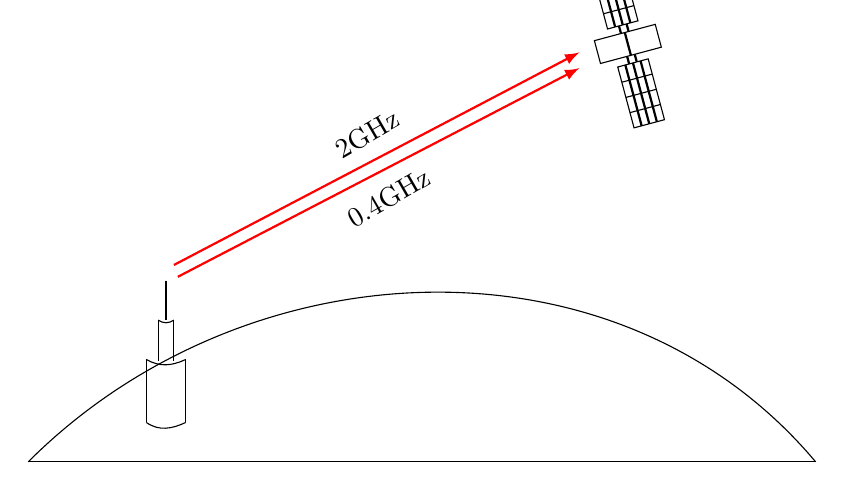
\begin{tikzpicture}
    \coordinate (lend) at (-5, 0);
    \coordinate (rend) at (5, 0);
    \draw (lend) to (rend);
    \draw (lend) to[out=45,in=-230] (rend);

    \coordinate (blb) at (-3.5, 0.5);
    \coordinate (brb) at (-3, 0.5);
    \draw (blb) to[out=-35,in=205] (brb);

    \coordinate (mlb) at (-3.5, 1.3);
    \coordinate (mrb) at (-3, 1.3);
    \draw (mlb) to[out=-30,in=205] (mrb);
    %\draw (mlb) to[out=35,in=-205] (mrb);
    \draw (blb) to (mlb);
    \draw (brb) to (mrb);
    
    \coordinate (tlb) at (-3.35, 1.8);
    \coordinate (trb) at (-3.15, 1.8);
    \draw (tlb) to[out=-35,in=215] (trb);
    \draw (tlb) to (-3.35, 1.28);
    \draw (trb) to (-3.15, 1.28);

    \coordinate (ulb) at (-3.26, 2.3);
    \coordinate (urb) at (-3.24, 2.3);
    \draw (ulb) to (-3.26, 1.8);
    \draw (urb) to (-3.24, 1.8);

    \rotatebox{15}{%
    \draw[] (3.5,4.6) rectangle (4.3,4.3);
    % Up panel
    \draw[thick] (3.9,4.3) to (3.9,4.6);
    \draw[thick] (3.85,4.6) to (3.85,4.7);
    \draw[thick] (3.95,4.6) to (3.95,4.7);
    \draw[] (3.7,5.5) rectangle (4.1,4.7);
    % grid
    \draw[thick] (3.8,4.7) to (3.8, 5.5); 
    \draw[thick] (3.9,4.7) to (3.9, 5.5); 
    \draw[thick] (4.0,4.7) to (4.0, 5.5); 
    \draw[] (3.7,4.9) to (4.1, 4.9);
    \draw[] (3.7,5.1) to (4.1, 5.1);
    \draw[] (3.7,5.3) to (4.1, 5.3);
    % Down panel
    \draw[thick] (3.85,4.3) to (3.85,4.2);
    \draw[thick] (3.95,4.3) to (3.95,4.2);
    \draw[] (3.7,3.4) rectangle (4.1,4.2);
    % grid
    \draw[thick] (3.8,3.4) to (3.8, 4.2); 
    \draw[thick] (3.9,3.4) to (3.9, 4.2); 
    \draw[thick] (4.0,3.4) to (4.0, 4.2); 
    \draw[] (3.7,3.6) to (4.1, 3.6);
    \draw[] (3.7,3.8) to (4.1, 3.8);
    \draw[] (3.7,4.0) to (4.1, 4.0);
    }
    
    \coordinate (satant1) at (2.0,  5.2);
    \coordinate (bcnant1) at (-3.15,2.5);
    \coordinate (satant2) at (2.0,  5.0);
    \coordinate (bcnant2) at (-3.10,2.35);
    \draw[thick,red,-latex] (bcnant1) -- node[above=1mm, align=center, black, rotate=30]{2GHz} (satant1);
    \draw[thick,red,-latex] (bcnant2) -- node[below=1mm, align=center, black, rotate=30]{0.4GHz} (satant2);

\end{tikzpicture}

\caption{DORIS System Description}
\label{fig:doris-system-description}
\end{figure}

\section{Theoretical Model of Doppler Observations}
According to \cite{lemoine-2016}, we define four basic events:
\begin{enumerate}
    \item beginning of emission of the 1\textsubscript{st} cycle by the emitter, 
    \(\tau_{e1}\) in the proper time scale of the emitter and \(t_1\) in the coordinate 
    time
    
    \item beginning of reception of the the 1\textsubscript{st} cycle by the receiver, 
    \(\tau_{r1'}\) in the proper time scale of the receiver and 
    \(t_{1'}\) in the coordinate time

    \item end of emission of the N\textsubscript{th} cycle by the emitter, 
    \(\tau_{e2}\) in the proper time scale of the emitter and \(t_2\) in the coordinate 
    time
    
    \item end of reception of the N\textsubscript{th} cycle by the receiver, 
    \(\tau_{r2'}\) in the proper time scale of the receiver and 
    \(t_{2'}\) in the coordinate time
\end{enumerate}

During the proper time interval \(\Delta\tau_{r} = \tau_{r2'} - \tau_{r1'}\), 
the receiver has received the \(N_e\) cycles sent by the emitter, with \(N_e = f_e \Delta\tau_e\), 
\(f_e\) being the proper frequency of the emitter. The receiver is also equipped with
an oscilator and during the proper time interval \(\Delta\tau_{r}\) has generated 
a number \(N_r = f_r \Delta\tau_r\) of cycles, \(f_r\) being the proper frequency of the 
receiver.

The Doppler measurement is the count, by the receiver electronics, of the number 
of cycles of difference between \(N_e\) and \(N_r\):
\begin{equation}
    \begin{split}
    N_{DOP} & = N_e - N_r\\
            & = f_e \Delta\tau_e - f_r \Delta\tau_r
    \end{split}
\end{equation}

\emph{In the RINEX files, this Doppler count is the difference between two phase measurements 
done at different time tags in the proper time-scale of the receiver.}

After a series of assumptions and simplifications, we can derive the theoretical 
formula for the Doppler count \cite{lemoine-2016}:
\begin{equation}
    \begin{split}
        \frac{c}{f_e \Delta\tau_r} N_{DOP} & \approx c \frac{f_e - f_r}{f_e} \\
        & - (1 - \frac{U_e}{c^2} - \frac{{V_e}^2}{2 c^2}) \frac{\rho_2 - \rho_1}{\Delta\tau_r}\\
        & + \frac{1}{c} (U_r - U_e + \frac{{V_r}^2 - {V_e}^2}{2}) \\
        & + \frac{2 \mu}{c^2 \Delta\tau_r} [\ln{(\frac{R_1 + R_{1'} + \rho_1}{R_1 + R_{1'} - \rho_1})} - \ln{(\frac{R_2 + R_{2'} + \rho_2}{R_2 + R_{2'} - \rho_2})}]
    \end{split}
\end{equation}

where \(U\) is the gravitational potential, \(V\) is the velocity of the clock, \(R\) 
is the geometric distance and \(\rho\) is the curvlinear trajectory (of the photon(s)).

The above equation can be (arbitrarily) split into two parts, one containing the ``measured'' 
quantities and one with the ``theoretical'' terms, as \cite{lemoine-2016}:
\begin{subequations}\label{eq:lem12}
  \begin{align}
    u_{measured} & = \frac{c}{f_e} (f_e - f_r -
     \frac{N_{DOP}}{\Delta\tau_r}) + \Delta u_{REL} \label{eq:lem12a} \\
    u_{theo}     &= \frac{\rho_2 - \rho_1}{\Delta\tau_r} (1- \frac{U_e}{c^2} - 
      \frac{{V_e}^2}{2 c^2}) \label{eq:lem12b}
  \end{align}
\end{subequations}

with
\begin{equation}
    \begin{split}
        \Delta u_{REL} &= \frac{1}{c} (U_r - U_e + \frac{{V_r}^2 - {V_e}^2}{2}) \\
        & + \frac{2 \mu}{c^2 \Delta\tau_r} [\ln{(\frac{R_1 + R_{1'} + \rho_1}{R_1 + R_{1'} - \rho_1})} - \ln{(\frac{R_2 + R_{2'} + \rho_2}{R_2 + R_{2'} - \rho_2})}]
    \end{split}
\end{equation}

We now need to introduce some additional corrections:
\(\Delta u_{IONO}\) and \(\Delta u_{TROPO}\), are the propagation corrections of 
the radio electric signal through the ionosphere and troposphere respectively. 

Additionaly, in the actual case (measurements), the nominal frequencies \(f_e\) and \(f_r\) 
are not the ``true'' ones; we hence need to apply a relative correction (e.g. for the 
emmiter) \(f_{e_T} = f_{e_N} (1 + \frac{\Delta f_e}{f_{e_N}})\), where the subscript \(T\) 
denotes the ``True'' frequency and \(N\) the nominal one. Thus in \ref{eq:lem12} the 
terms \(f_e\) and \(f_r\) need to be substituted by \(f_{e_T}\) and \(f_{r_T}\) respectively.

We will place \(\Delta u_{IONO}\) and \(\Delta u_{REL}\) (which do not involve adjusted parameters) 
on the ``measured'' part of \ref{eq:lem12} and \(\Delta u_{TROPO}\) and \(\frac{\Delta f_e}{f_{e_N}}\) 
on the ``theoretical'' part; neglecting some minor terms, we reach the equation \cite{lemoine-2016}:
\begin{subequations} \label{eq:lem13}
    \begin{align}
        u_{measured} & = \frac{c}{f_{e_N}} (f_{e_N} - f_{r_T} -
          \frac{N_{DOP}}{\Delta\tau_r}) + \Delta u_{REL} + 
          \Delta u_{IONO} \label{eq:lem13a} \\
        u_{theo} &= \frac{\rho_2 - \rho_1}{\Delta\tau_r} 
          (1- \frac{U_e}{c^2} - \frac{{V_e}^2}{2 c^2}) + 
          \Delta u_{TROPO} - \frac{c(\frac{N_{DOP}}{\Delta\tau_r} + 
          f_{r_T})}{f_{e_N}} \frac{\Delta f_e}{f_{e_N}} \label{eq:lem13b}
    \end{align}
\end{subequations}

where 
\begin{itemize}
    \item \(u_{measured}\) is the measured relative velocity between the emitter and 
    the receiver between the events 1' and 2', based on the Doppler count \(N_{DOP}\), 
    corrected for the ionospheric and relativistic effects.

    \item \(u_{theo}\) is the the theoretical (computed) emitter/receiver relative velocity 
    between the events 1' and 2', corrected for the tropospheric effect and for a solved-for 
    frequency bias \(\frac{\Delta f_e}{f_{e_N}}\) of the emitter. \(f_{r_T} = f_{r_N} (1 + \frac{\Delta f_r}{f_{r_N}})\) 
    is an estimate of the proper frequency of the receiver.

    \item \(\Delta u_{REL} = \Delta u_{{REL}_c} + \Delta u_{{REL}_r}\) is the relativistic 
    correction, composed of two parts: the clock correction \(\Delta u_{{REL}_c}\) and the 
    travel correction \(\Delta u_{{REL}_r}\)
    \begin{subequations} \label{eq:lem14}
        \begin{align}
            \Delta u_{{REL}_c} & = \frac{1}{c} 
              (U_r - U_e + \frac{{V_r}^2 - {V_e}^2}{2}) \label{eq:lem14a}\\
            \Delta u_{{REL}_r} & = \frac{2 \mu}{c^2 \Delta\tau_r} \left[ 
              \ln{(\frac{R_1 + R_{1'} + \rho_1}{R_1 + R_{1'} - \rho_1})} - 
              \ln{(\frac{R_2 + R_{2'} + \rho_2}{R_2 + R_{2'} - \rho_2})} \right] \label{eq:lem14b}
        \end{align}
    \end{subequations}
\end{itemize}

Note that \ref{eq:lem13} can be further simplified to \ref{eq:lem17} by 
ommiting small terms (\ref{ssec:small-terms}).

\emph{Usually, one frequency offset and one tropospheric zenithal bias are adjusted per pass.}

\section{Implementation of the Doppler Observation Model}

\subsection{Small Terms}
\label{ssec:small-terms}

In \ref{eq:lem13}, the smallest terms are \(-U_e / c^2 - {V_e}^2 / 2 c^2\) and 
\(\Delta u_{{REL}_T}\); in the case of DORIS they ammount to \num{11.} and 
\num{6.} \SI{10e-6}{\meter\per\second} respectively (\cite{lemoine-2016}). 
Furthermore, since the emitters are located on the ground, the term 
\(-U_e / c^2 - {V_e}^2 / 2 c^2\) is constant per station. This small 
relativistic offset is absorbed by the adjustment of \(\Delta f_e / f_{eN}\). 
So it is possibly to furher simplify \ref{eq:lem13} to:
\begin{subequations} \label{eq:lem17}
    \begin{align}
        u_{measured} & = \frac{c}{f_{e_N}} (f_{e_N} - f_{r_T} -
          \frac{N_{DOP}}{\Delta\tau_r}) + 
          \Delta u_{{REL}_C} + \Delta u_{IONO} \label{eq:lem17a}\\
        u_{theo} &= \frac{\rho_2 - \rho_1}{\Delta\tau_r} + \Delta u_{TROPO} - 
          \frac{c(\frac{N_{DOP}}{\Delta\tau_r} + f_{r_T})}{f_{e_N}} 
          \frac{\Delta f_e}{f_{e_N}} \label{eq:lem17b}
    \end{align}
\end{subequations}

\subsection{Correction of Aberration}

\subsection{Geopotential}
For a station on the geoid, the potential at the level of the station is the sum 
of the gravitational potential and the centrifugal potential due to the Earth's 
rotation: \(U_{GEO} = U_e + \frac{{V_e}^2}{2}\), which is a constant. For a station 
not located on the geoid, the quantity \(U_e + \frac{{V_e}^2}{2}\) will only depend 
on the height of the beacon above the geoid.

For the computation of the gravitational potential for \gls{leo} satellites, 
the pottential \(U_r\) cannot be restricted to the central term only and we must 
take into account the \(J_2\) term (at least, in addition to \(\mu / r\). The formula 
for the computation of the potential in this case is \cite{lemoine-2016}:
\begin{equation}
  \label{eq:lem18}
  U_r = \frac{\mu}{r} \left( 1- \left(\frac{\alpha_\Earth}{r}\right)^2 
    J_2 \frac{3 sin^2(\phi) - 1}{2} \right)
\end{equation}
with \(\alpha_\Earth\) the equatorial radious of the earth, \(r\) radial 
distance of the satellite (to the Earth's center), \(\phi\) latitude of the 
satellite and \(J_2 = 1.0826359 \dot 10^{-3}\) in the zero-tide system.

\subsection{True Proper Frequency of the Receiver}
\label{ssec:true-proprtfrequency-of-the-receiver}

For the term \(f_{r_T}\) that appears in \ref{eq:lem13}, we need an estimate of \(\Delta f_{r} / f_{r_N}\). 
This estimate can be obtained in one of the following ways \cite{lemoine-2016}:
\begin{enumerate}
    \item via the field ``F'' recorded for every single measurement in the DORIS 
    RINEX file (see \ref{ssec:relative-frequency-offset}); not that this estimation 
    is not very smooth, as noticed by \cite{GAO2015} and it is advisable, before 
    using it in \ref{eq:lem13}, to perform a linear (or polynomial) regression of 
    these estimates over one or a few days.

    \item It can also be obtained from a polynomial regression
    over the frequency offsets estimated during the passes
    over the master beacons

    \item It can finally be estimated by the users themselves as a
    by-product of their re-computation of the timetagging polynomial (see \cite{MERCIER2010})
\end{enumerate}

\subsection{Ionospheric Correction}
A first-order iono-free pseudo-range measurement on the \SI{2}{\GHz} channel is built by combining
the \SI{400}{\MHz} and \SI{2}{\GHz} measurements in the following way:
\begin{equation}
  C_{iono-free-2GHz} = \frac{\gamma C_{2GHz} - C_{400MHz}}{\gamma - 1}
\end{equation}
where \(\gamma\) is the square of the frequency ratio: 
\(\gamma = {(\frac{f_{2GHz}}{f_{400MHz}})}^2\).

Converting to iono-free phase measurement on the \SI{2}{\GHz} channel using 
\(c\)  the speed of light and \(L_{\alpha}\) is the phase measurements on the 
\(\alpha\) channel (\(\alpha\) = \SI{2}{\GHz} or \SI{400}{\MHz}), we get:

\begin{equation}
  \begin{aligned}
  L_{iono-free-2GHz} &= \frac{\gamma L_{2GHz} - 
    \sqrt{\gamma}L_{400MHz}}{\gamma - 1} \\
                     &= L_{2GHz} + \frac{L_{2GHz} - 
                        \sqrt{\gamma}L_{400MHz}}{\gamma - 1}
  \end{aligned}
\end{equation}

The coordinates of the iono-free phase centers are given by the following formula:
\begin{equation}
  \vec{\bm{r}}_{iono-free-2GHz} = \frac{\vec{\bm{r}}_{400MHz,2GHz}}{\gamma - 1}
\end{equation}
where \(\vec{\bm{r}}_{iono-free-2GHz}\) is the vector from the \SI{2}{\GHz} 
phase center to the iono-free phase center and \(\vec{\bm{r}}_{400MHz,2GHz}\) 
is the vector from the \SI{400}{\Hz} to the \SI{2}{\GHz} phase center. In 
DORIS, the iono-free phase centers are located a few mm away from the 
\SI{2}{\GHz} phase centers, in the direction opposite to the \SI{400}{\MHz} 
phase centers.
